\chapter{Conclusions}
\label{chapter:Conclusion}
\thispagestyle{myheadings}

% set this to the location of the figures for this chapter. it may
% also want to be ../Figures/2_Body/ or something. make sure that
% it has a trailing directory separator (i.e., '/')!
\graphicspath{{3_Conclusion/Figures/}}


\section{ Potential cellular mechanisms for reinforcement learning}

The results described in  \textit{Chapter 4}  \& \textit{Chapter 5} indicate that HVC operates on two distinct levels: a mesoscopic level that is highly stable and a microscopic level where individual neurons are free to change their participation. It is possible that HVC may represent learned behaviors in the stability of network patterns that persist in spite of the drifting participation of individual neurons. The instability of the neural program could reflect the microscopic day-to day changes in song, but the difference in magnitude raises the question: If this drift is truly random, why does the song not undergo larger shifts? What explains the persistence of the song motor pattern in spite of the unstable projection neurons underlying song? What drives the instability of single neurons? Potentially, this fine scale plasticity we observe may reflect an underlying mechanism that is important for maintaining the stability of the motor behavior over time. It is possible that fine-scale drift may somehow actively serve as a mechanism for memory maintenance and motor stability.

Given that HVC receives inputs from the auditory system (Akutagawa and Konishi, 2010; \cite{Vates1995-zr}, it is an accommodating location for sensorimotor integration.  HVC sits atop both the AFP and the VMP, evaluations of prediction-errors here would provide a convenient mechanism to mediate sensory-motor learning- and could provide the site of active maintenance of the song motor program throughout adulthood. However, many experimental findings have reduced the likelihood of this being true. Deafened birds do not show significantly altered HVC responses during singing. In the canary, auditory responses cannot be elicited in HVC until seconds after song has ended. Intracellular recordings in HVC$_{X}$ neurons have failed to find even sub-threshold changes in response to auditory stimuli that overlap with song production. \cite{Hamaguchi2014-sx}. Together, this suggests that HVC projection neurons likely have no real-time mechanisms for updating the motor code in response to sensory feedback.  However, our findings provide valuable insight- the changes we observe typically do not occur during the day, but discretely over periods of sleep. This suggests that there may be 'offline' mechanisms that update the motor plan. The premotor nucleus HVC might still serve as a structure where auditory feedback is ultimately integrated by constant fine-tuning of song motor commands, where individual cells adapt their firing times to regulate the behavioral output of song after the accumulation and evaluation performance errors across the course of a day. In this way, drifting excitatory neurons may be hedonistic; changing their activity based on a history of activity that led to 'good' performances, stabilized by mesoscopic inhibition (Zagha, Ge, and McCormick 2015). However, these changes may simply be the result of intrinsic homeostatic mechanisms that support network stability.


In this concluding section, I propose experiments that could address if changes in neural participation is important to memory stability or maintenance.  A key question is whether drift at the single neuron level is influenced by an animal's perceived behavioral performance. These experiments hold the potential to reveal single neuron rules underlying sensory-motor learning and address long standing questions about the nature of memory stability for skilled movements.

\section{ Engineering limitations, and future directions.}
\subsection{ Identifying the downstream projection targets of projection neurons during imaging }


 How do different projection neuron classes contribute to the stability of the motor program? 
One of the key limitations of the imaging studies performed in the previous chapters is that we could not segregate the downstream projection targets of the neurons we recorded from. While HVC projection neurons all appear to be discretely active at one or a few moments of song, these neurons are a heterogeneous population. They differ greatly in their morphology, and send their axons to opposite ends of the brain. HVC$_{X}$ and HVC$_{RA}$ possibly send independent computational contributions to the AFP and the VMP- if drift occurs in one population but not the other, it would have very different implications. It is clearly important to undertake experiments that can identify cell-type specific contributions to neural coding. There are two major challenges. First, we lack a precise way of genetically labeling distinct HVC projection neuron subpopulations. Secondly, we are limited in both the resolution and the bandwidth of our miniature head-mounted microscopes. I briefly describe how to address these challenges below.
 

\subsubsection{ Genetic Labeling of specific subpopulations}
While the zebra finch genome has been sequenced and several transgenics have been generated \cite{Scott:2005gr}, viral transduction in the songbird remains a challenge, and there are limited genetic tools currently available. While excitatory neurons in HVC can be preferentially targeted for genetic manipulation, it is still not possible to target specific sub-populations using cell type specific promoters. However, the nucleated structure of the songbird brain makes it ideal for intersectional strategies using retrograde labeling. Preliminary data suggests that it is possible to selectively image from populations of cells of a known origin using retrograde viruses (Figure 6$\cdot$1). New advances in blood based viruses and advanced retrograde viruses could spur advances as well.

\begin{figure}[!htb]
 %\begin{minipage}[t]{0.49\linewidth}\centering
    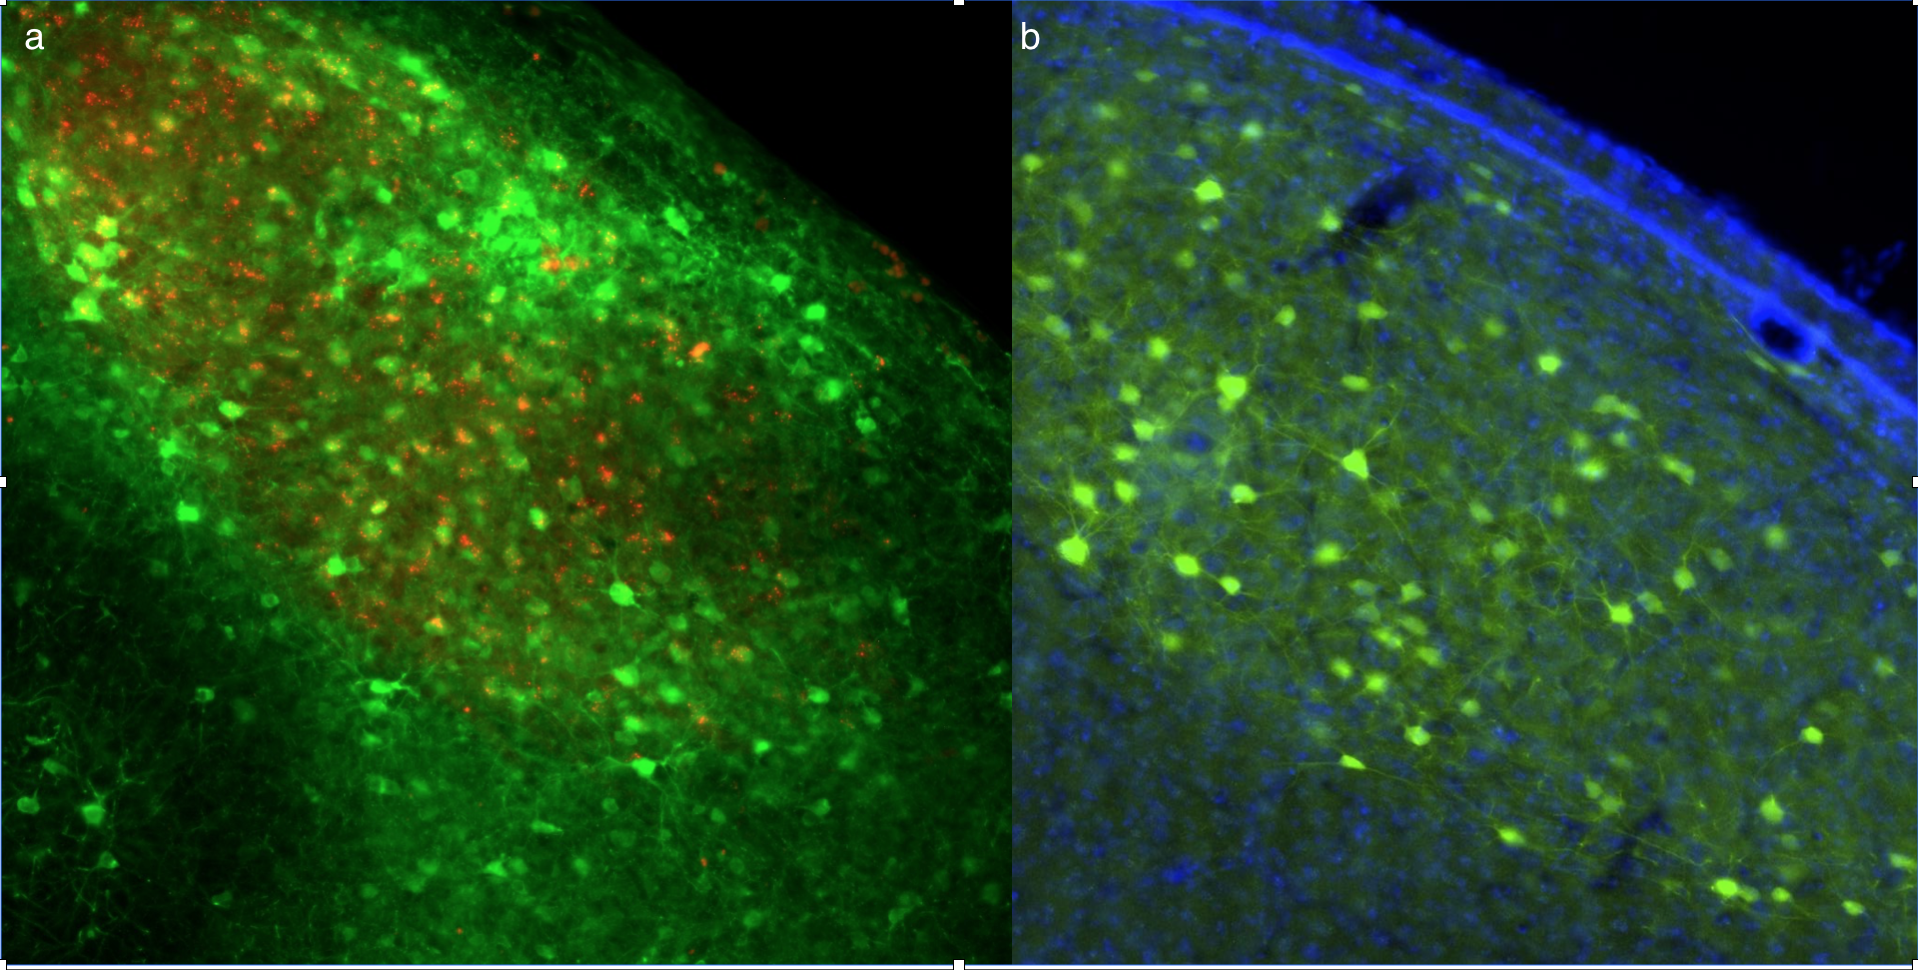
\includegraphics[width=12cm]{figure2.png}
    \centering
\medskip
\caption[Cell-type specific genetic labeling]{\footnotesize  \textbf{Cell-type specific genetic labeling} \textbf{a}, \textit{Left,} Lentiviral infection of a heterogeneous mixture of neurons in HVC \textit{Right,} HVC-X labeling using retrograde viruses. Red  = DiI, Green = GCaMP6, Blue = DAPI }

\label{fig:Sampling}
\end{figure}



Even without adopting new genetic tools, one could simultaneously image a retrogradely injected dye (for example, DiI; which has green excitation and red emission) and the GCaMP6, so that projection neuron subtypes in songbirds can be identified, based on the presence or absence of retrograde labeling from downstream nuclei.  However, current  miniscope designs can only image in one band/wavelength ( In our case, we use blue excitation and green emission).
  
\subsubsection{ Multicolor Imaging}
Single photon imaging with miniature head-mounted fluorescence microscopes has become an increasingly widespread and powerful method for recording neural activity in freely moving animals at the cellular-level.
In our hands, it has been indispensable in describing the stability and spatial organization of single projection neurons- but in many ways, this technique still remain relatively limited. Due to bandwidth constraints, it is not possible to  use different fluorophores to segregate signals by cell type or projection target. One way to address this is to make modifications to incorporate two or more independent color channels.For example, microscopes could be designed with multi-peaked excitation LEDs and color cameras, and paired with the appropriate filter sets that accommodate multi-color imaging in blue/green and green/red. This strategy could increase the bandwidth of information gathered within the imaging plane- and allow the use of additional fluorescent proteins or tracers to disambiguate specific neuron types within an imaging field (Figure 6$\cdot$2).

 \begin{figure}[!htb]
 %\begin{minipage}[t]{0.49\linewidth}\centering
    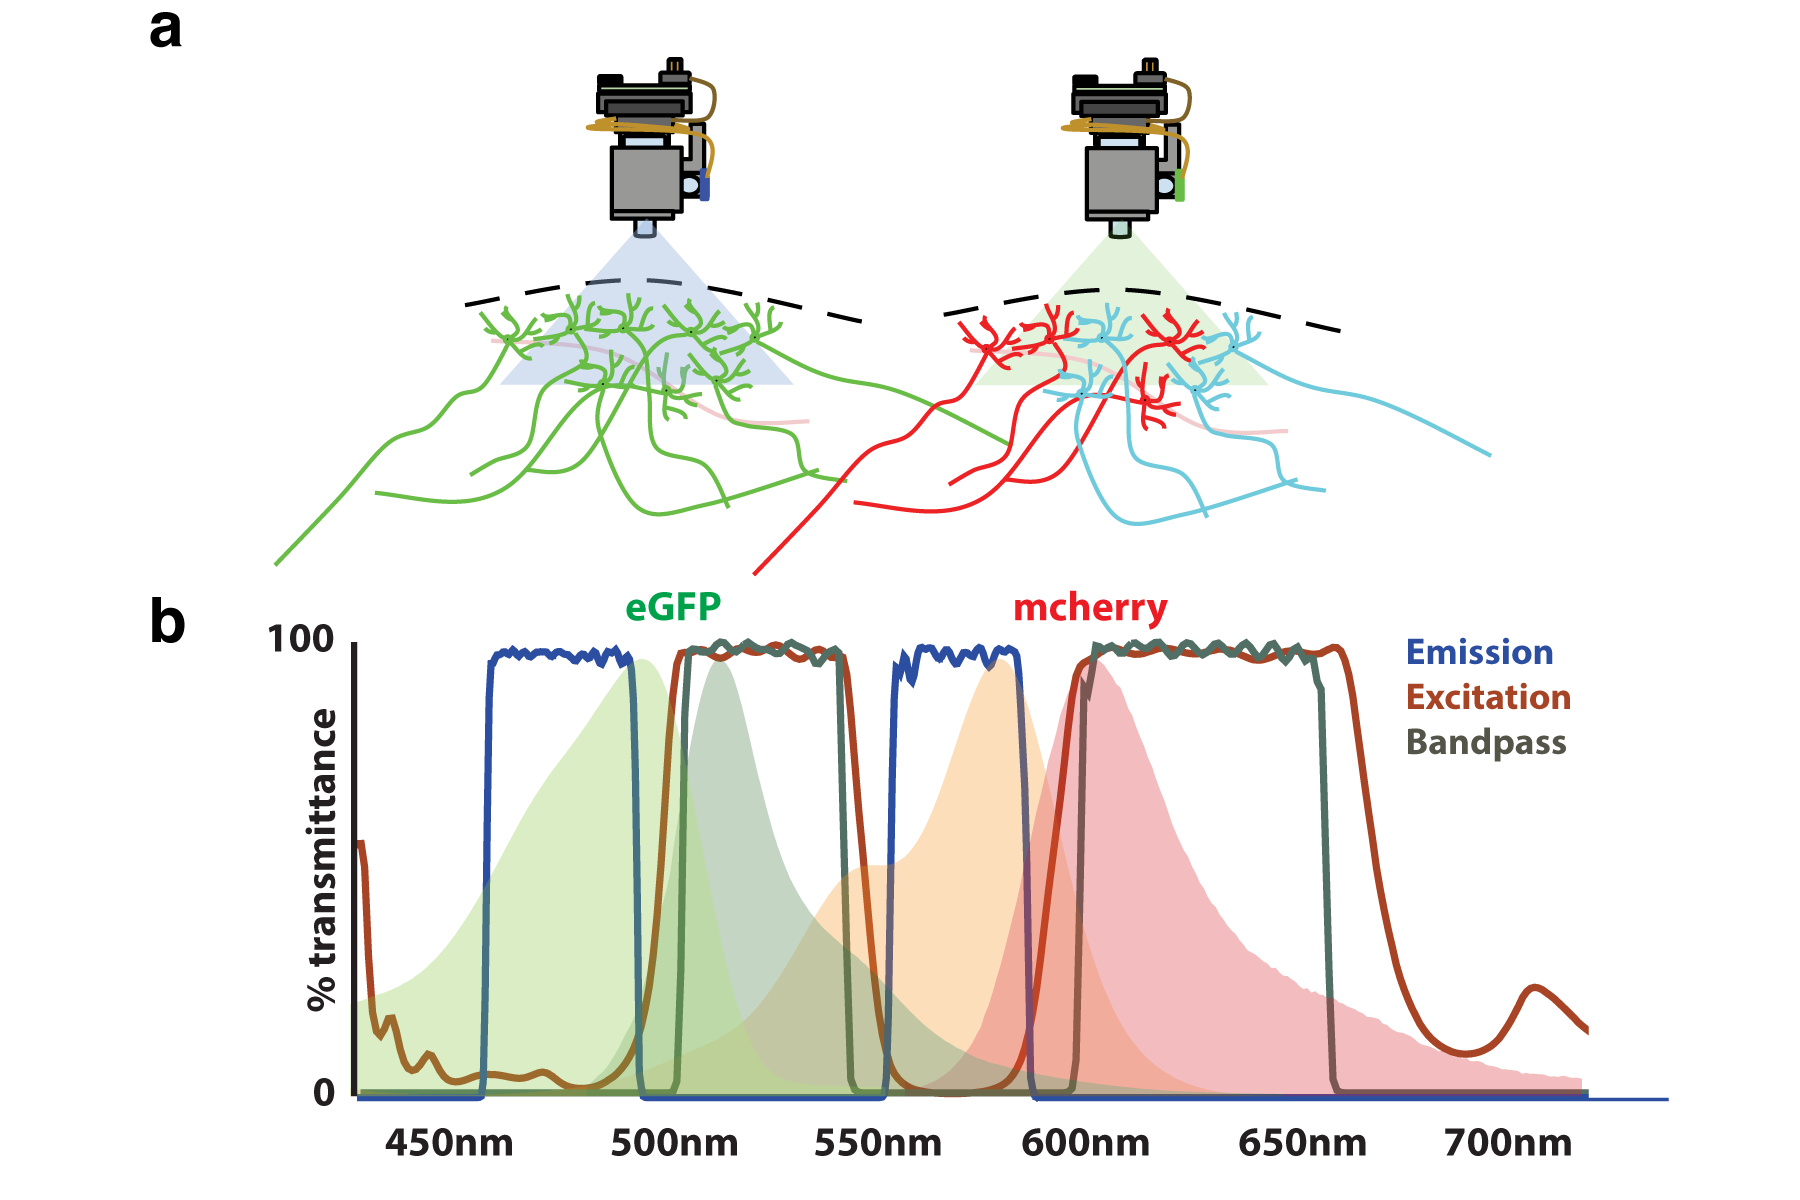
\includegraphics[width=13cm]{figure3.png}
    \centering
\medskip
\caption[Multi-wavelength imaging in a 1P miniature microscope.]{\footnotesize  \textbf{Multi-wavelength imaging in a 1P miniature microscope.}  \textbf{A} dual color microscopes can be used to disambiguate populations of neurons using a combination of genetically encoded reporters, or injected dies. \textbf{B} Dual pass band filter sets are commercially available, and are well suited to this application. }

\label{fig:Sampling}
\end{figure}



\subsection{Structured Illumination Microscopy} 

Another limitation to single photon imaging is that the poor z-axis resolution can make it difficult to disambiguate signals coming from overlapping cells. While computational techniques have emerged that are designed to de-mix overlapping neurons, these techniques are still highly parameterized  and need to be optimized per preparation \cite{Picardo:2016hv}. To date, the axial resolution of bench-top multi-photon microscopy is still vastly superior to that which can be achieved otherwise. In spite of these limitations, head-mounted microscopes are often the only way to optically observe neural populations during naturalistic behaviors. In the songbird, we have observed that head-fixation is an extremely stressful experience. Under this condition, birds rarely sing. To promote song production, birds are deprived of water and social exposure to females- and these are used as an incentive to sing.  As a result, this paradigm likely impedes the study of 'undirected' singing in songbirds, a learning-intensive form of song practice in the zebra finch. We have evidence that excitatory neuron activity during the production of undirected song can differ from directed, and that network exploration during song 'practice' may be important. (Figure 6$\cdot$3)   

 \begin{figure}[!htb]
 %\begin{minipage}[t]{0.49\linewidth}\centering
    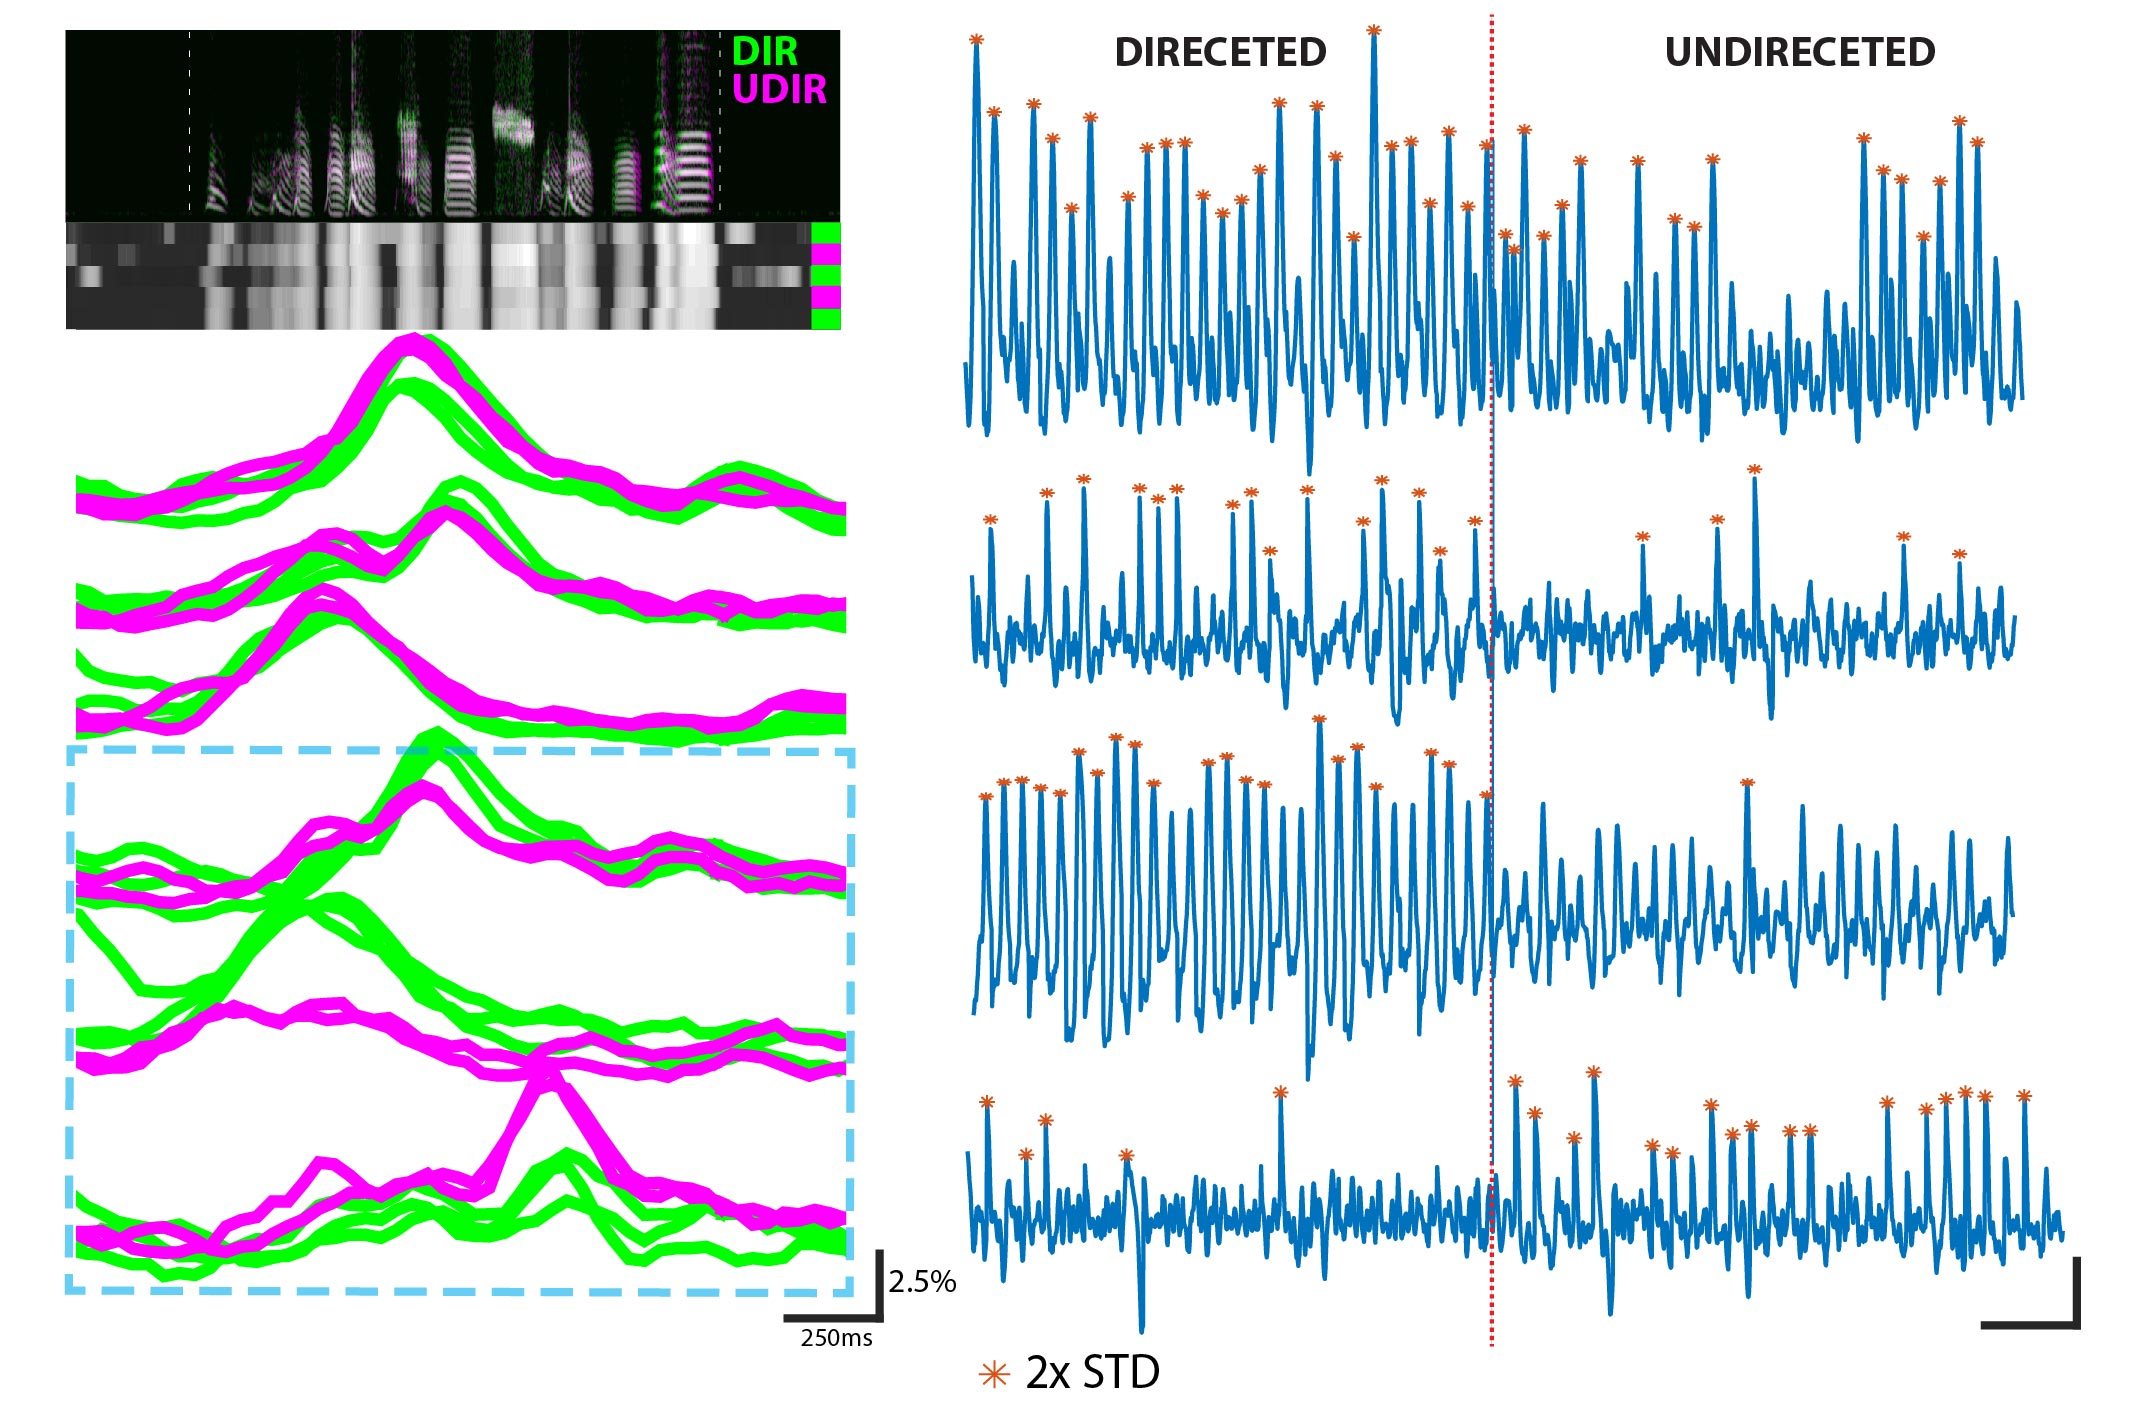
\includegraphics[width=11cm]{figure5.jpg}
    \centering
\medskip
\caption[Context related changes in HVC projection neurons ]{\footnotesize  \textbf{Context related changes in HVC projection neurons} Head-fixing animals may preclude the study of differences in motor coding that relate to the behavioral context of the animal. We see some evidence that motor codes that underlie song that is 'directed' to a female may differ from when song is produced in isolation.  \textit{Left,} Several ROIs aligned to song, from interleaved trials of directed and undirected song. Blue dotted-line inset highlights several ROIs the show some differences related to behavioral context. (Green = Directed, Magenta = undirected) \textit{Right,} fluorescent time series data from several ROIS, concatenated from many songs in each context. Differences in peak participation frequency in each context suggest that variabilities in coding may exist as a function of behavioral context.}

\label{fig:Sampling}
\end{figure}

 \begin{figure}[!htb]
 %\begin{minipage}[t]{0.49\linewidth}\centering
    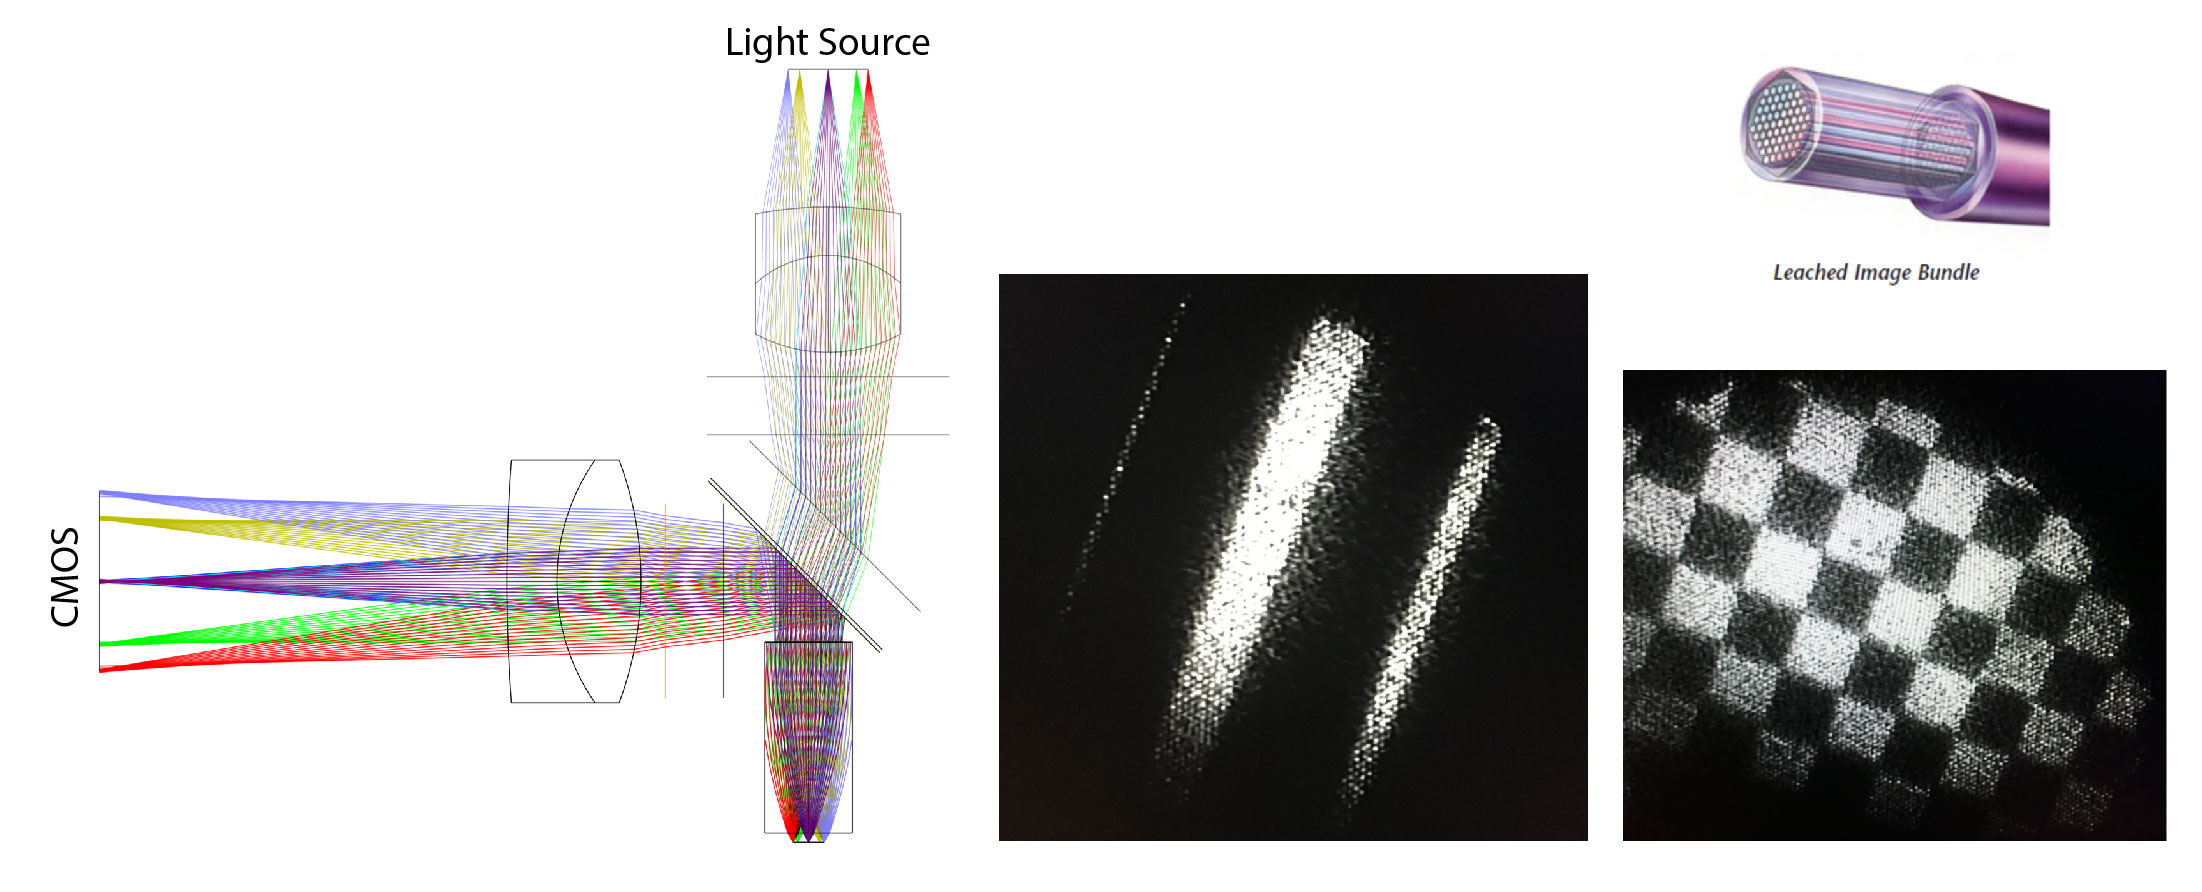
\includegraphics[width=11cm]{figure4.jpg}
    \centering
\medskip
\caption[Structured Illumination Integration]{\footnotesize  \textbf{Structured Illumination Integration} The integration of structured illumination into miniature microscopes would improve z-axis resolution, and could allow for arbitrary or patterned stimulation- creating all-optical interrogation, at the single cell level, in a freely behaving animal. \textit{Left,} Light-path for SIM integration. \textit{Right}, DMD patterns on the coherent fiber.}

\label{fig:Sampling}
\end{figure}
  
Compared to these laser scanning techniques, single photon imaging has relatively poor depth of field, z-axis sectioning, and tissue penetration. These issues can potentially be addressed using optical and computational techniques that improve signal quality by rejecting unwanted noise. The most promising of these techniques is Structured Illumination Microscopy (SIM). The increase in resolution from SIM is obtained by providing non-uniform excitation light patterns that feature sinusoidal intensity variations in one or more dimensions coupled with powerful image reconstruction techniques. This allows the rejection of out of focus light from outside of the image plane, at the expense of decreasing the effective frame-rate due to the computational step. Using micro LEDs and/or DMD coupled laser light deliver through coherent fiber bundles, SIM can be delivered through a custom designed miniature microscope. In preliminary experiments, a Digital Micro-mirror Device (Texas Instruments LightCrafter) is used to create three grid patterns that are shifted by a third of the period. After acquiring the three images, the sectioned image is computed and background fluorescence is rejected.  Extensions to this strategy could afford new ways to control neurons in freely behaving animals, using patterned illumination for optical control of spatially segregated neurons, and potentially could afford 3D volumetric imaging (Szabo et al. 2014). (Ventalon et al. 2015). Proof-of-concept work is currently occurring in an on-going collaboration with Bernardo Sabatini's lab in Harvard Medical School. Figure 6$\cdot$4 A fast cycle of ZEMAX optical path modeling and re-printing of the microscope housing has facilitated this collaborative engineering project, and has already demonstrated improvements in the rejection of out-of-plane fluorescence.





\section{ROI based, near-Real-Time Brain Machine Interface (BMI) experiments }


Motivated by the observation that the stability of song memory is rooted in the stability of network patterns that persist in spite of drifting individual neuron dynamics, we hope to explain the persistence of the song motor pattern in spite of unstable projection neurons. It is experimentally possible to directly test the hypothesis that changes in the firing patterns of single neurons in pre-motor cortex is beneficial to the motor program. I propose to explicitly test if the activity of these cells is shaped by the recent history of time-correlated reward or punishment signals, by using real-time Brain Machine Interfacing (BMI) experiments 
 
What is the utility of drifting motor commands in the production of a stable motor behavior? Previous studies using extracellular and intracellular recordings indicate that during vocal production,  HVC$_{X}$ and HVC$_{RA}$ neurons are insensitive to feedback perturbations, suggesting that performance evaluation does not occur in these cells during song. However, spine imaging studies have found that deafening shrinks and destabilizes dendritic spines on HVC$_{X}$ neurons within 12-48 hr and that these changes precede and predict the severity of song degradation. 


These results suggest that at least HVC$_{X}$ cells are sensitive to auditory feedback on the same timescale that we have observed drifting firing patterns. The descending projections of HVC$_{X}$ (and possibly HVC$_{AV}$) possibly  relay an efference copy of the motor control sequences that could be evaluated alongside song performance in the basal ganglia. In this case, we might expect some mechanism would exist at the interface of auditory and motor generation systems to consolidate and reconcile this evaluation. Perhaps  HVC serves as a structure where auditory feedback is ultimately integrated by constant fine-tuning of song motor commands. Individual cells slightly adapt their firing times to regulate the behavioral output of song after the accumulation and evaluation of performance errors, forming the mechanistic basis of memory maintenance and and motor stability. 


This could be tested using a variant of CAF where the auditory feedback is made contingent on the activity of single HVC, LMAN, or Area X neuron (Figure 6$\cdot$5). The aim would be to steer plasticity in cells that are already under observation. In this paradigm the bird can only escape aversive white noise playback by modulating the firing rate of either a single isolated unit, or group of units (Koralek et al. 2012) Potentially, this drift will be modulated by performance errors delivered through conditional auditory feedback and consolidated over periods of sleep.  This drift could be blocked or reduced by selective blockage of the output structures of the basal ganglia.
				
This use of region of interest (ROI) based feedback could be contingent on one or several neurons, and could be contrasted by feedback contingent on specific times in song in order to tease apart the individual contributions of individual cell types in HVC- although this strategy could be deployed across the song system. It would be critical to characterize the response of different cell types within a day, as well as the responses across days, to this feedback contingency in order to tease apart the cell-type specific mechanisms of motor adaptation. It would be equally interesting to monitor spontaneous activity during sleep, to observe what offline dynamics may be occurring that may predict changes or reinforce stable cells.

 
 \begin{figure}[!htb]
 %\begin{minipage}[t]{0.49\linewidth}\centering
    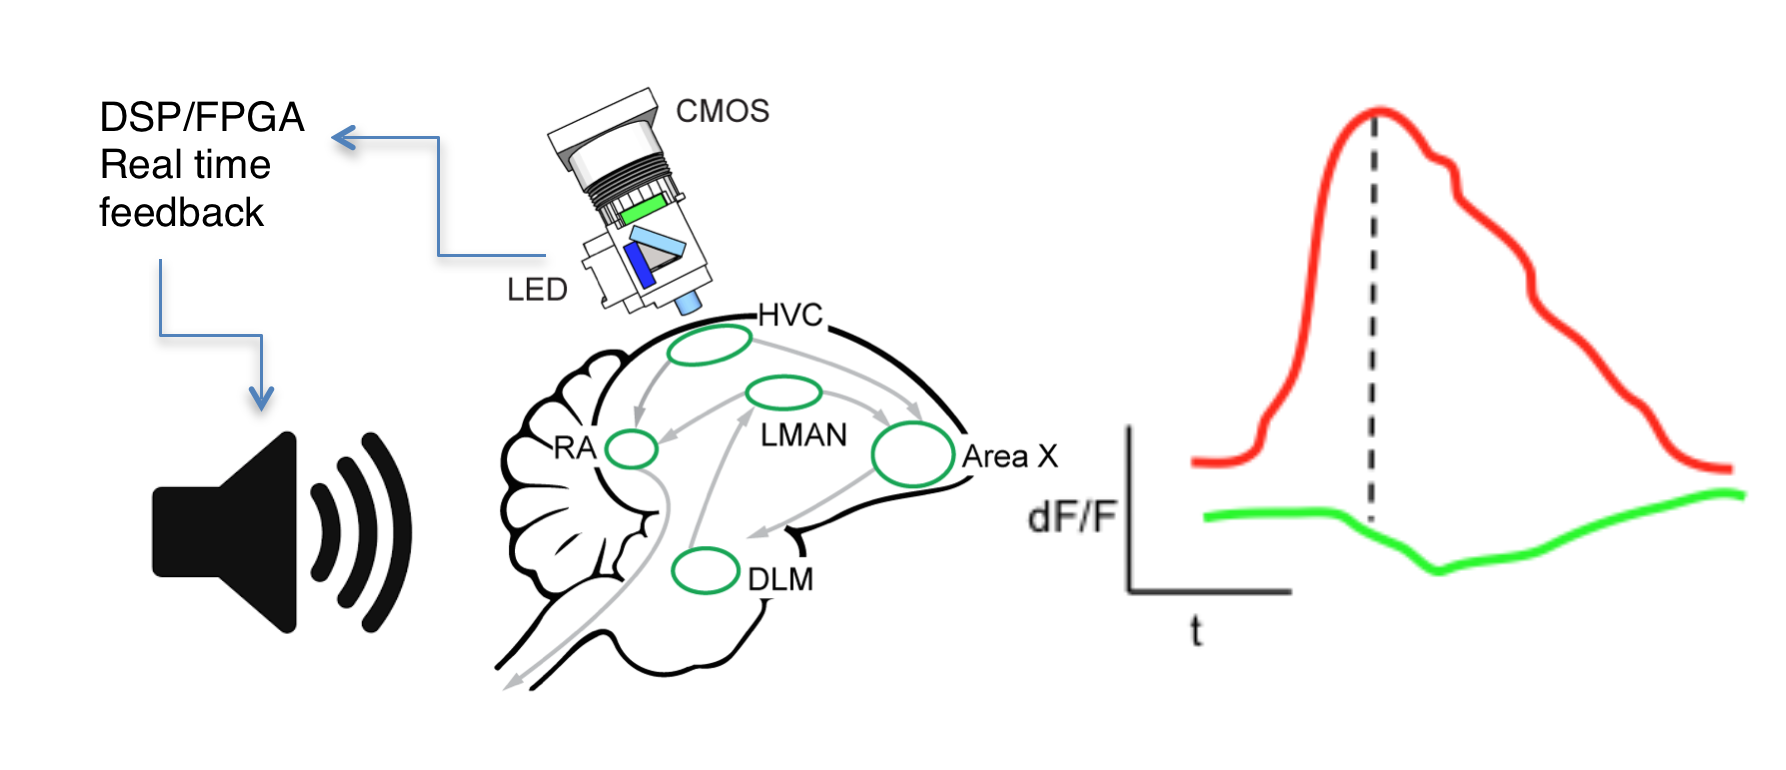
\includegraphics[width=11cm]{figure1.png}
    \centering
\medskip
\caption[BMI experimental outline]{\footnotesize  \textbf{BMI experimental outline} \textbf{a}, \textit{Left,} To perform experiments that can identify neural activity patterns in real time, the video stream is constantly processed to extract fluorescence information in pixels within predefined regions of interest. Rules (such as the ratio of activity in two ensembles) are applied to this near-real-time ROI analysis to trigger external events through a programmable digital output, such as white noise contingent on the pattern of activity recorded through the head-mounted microscope. In this mode, the camera provides a near-real-time brain machine interface allowing songbirds to control sounds directly through the measured calcium signals in the brain. Other BMI possibilities include closed-loop stimulation experiments that seek to electrically or optically disrupt patterns of activity in real-time.}
\label{fig:Sampling}
\end{figure}
 
 
 
 \section{The role of sleep}
The role of sleep, as it relates to motor systems, is not well-known. Chapter 5 describes changes in neural patterns that discretely occur overnight, raising the possibility that new patterns of activity 'invented' over intervals of sleep provide important raw material for song learning and maintenance. Francis Crick proposed that noisy reactivation of neural circuits in sleep weakens the strongest pathways in the brain, promoting adaptive plasticity. This leads us to ask: Do new strategies of motor exploration occur over periods of sleep, seeking the source of variability and motor-sequence exploration both during periods of song and during 'offline' periods? It is possible that spontaneous activity patterns in sleep allow injection of randomness that allows for fine grade motor exploration through subtle changes in synaptic weights. This may be visualized in large scale changes seen across days, which may be guided or biased within a day by small populations of auditory and/or context sensitive neurons. 
 
Sleep is widely believed to be important for learning and memory, particularly in the process of consolidation, a process that transforms short-term memories into more stable longer-term memory representations (Kuriyama, Stickgold, and Walker 2004)  (Walker and Stickgold 2004)  (Stickgold and Walker 2004)  (Diekelmann and Born 2010). Many theoretical models propose that consolidation would benefit from sleep, suggesting that sleep prevents the possible interference of daily activities on memory consolidation (Diekelmann and Born 2010). However, experimental evidence explicitly demonstrates that this process is sparse. 

Learning new tasks is often associated with stabilization of ensemble activity patterns across days as well as increased task-related neuronal activity. The emerging picture is that neuronal representations are explored by behavioral relevance during the day, but that long-term integration of beneficial changes occurs during offline periods. This 'consolidation' may  transform short-term optimal network configurations, that may be inherently fragile and plastic, into more stable and long-term stored memory representations without the interference of online processes (Ferry and McGaugh 2000; Izquierdo and McGaugh 2000)  (Eisenberg and Dudai 2004) (Diekelmann and Born 2010) (Diekelmann and Born 2010)

 \begin{figure}[!htb]
 %\begin{minipage}[t]{0.49\linewidth}\centering
    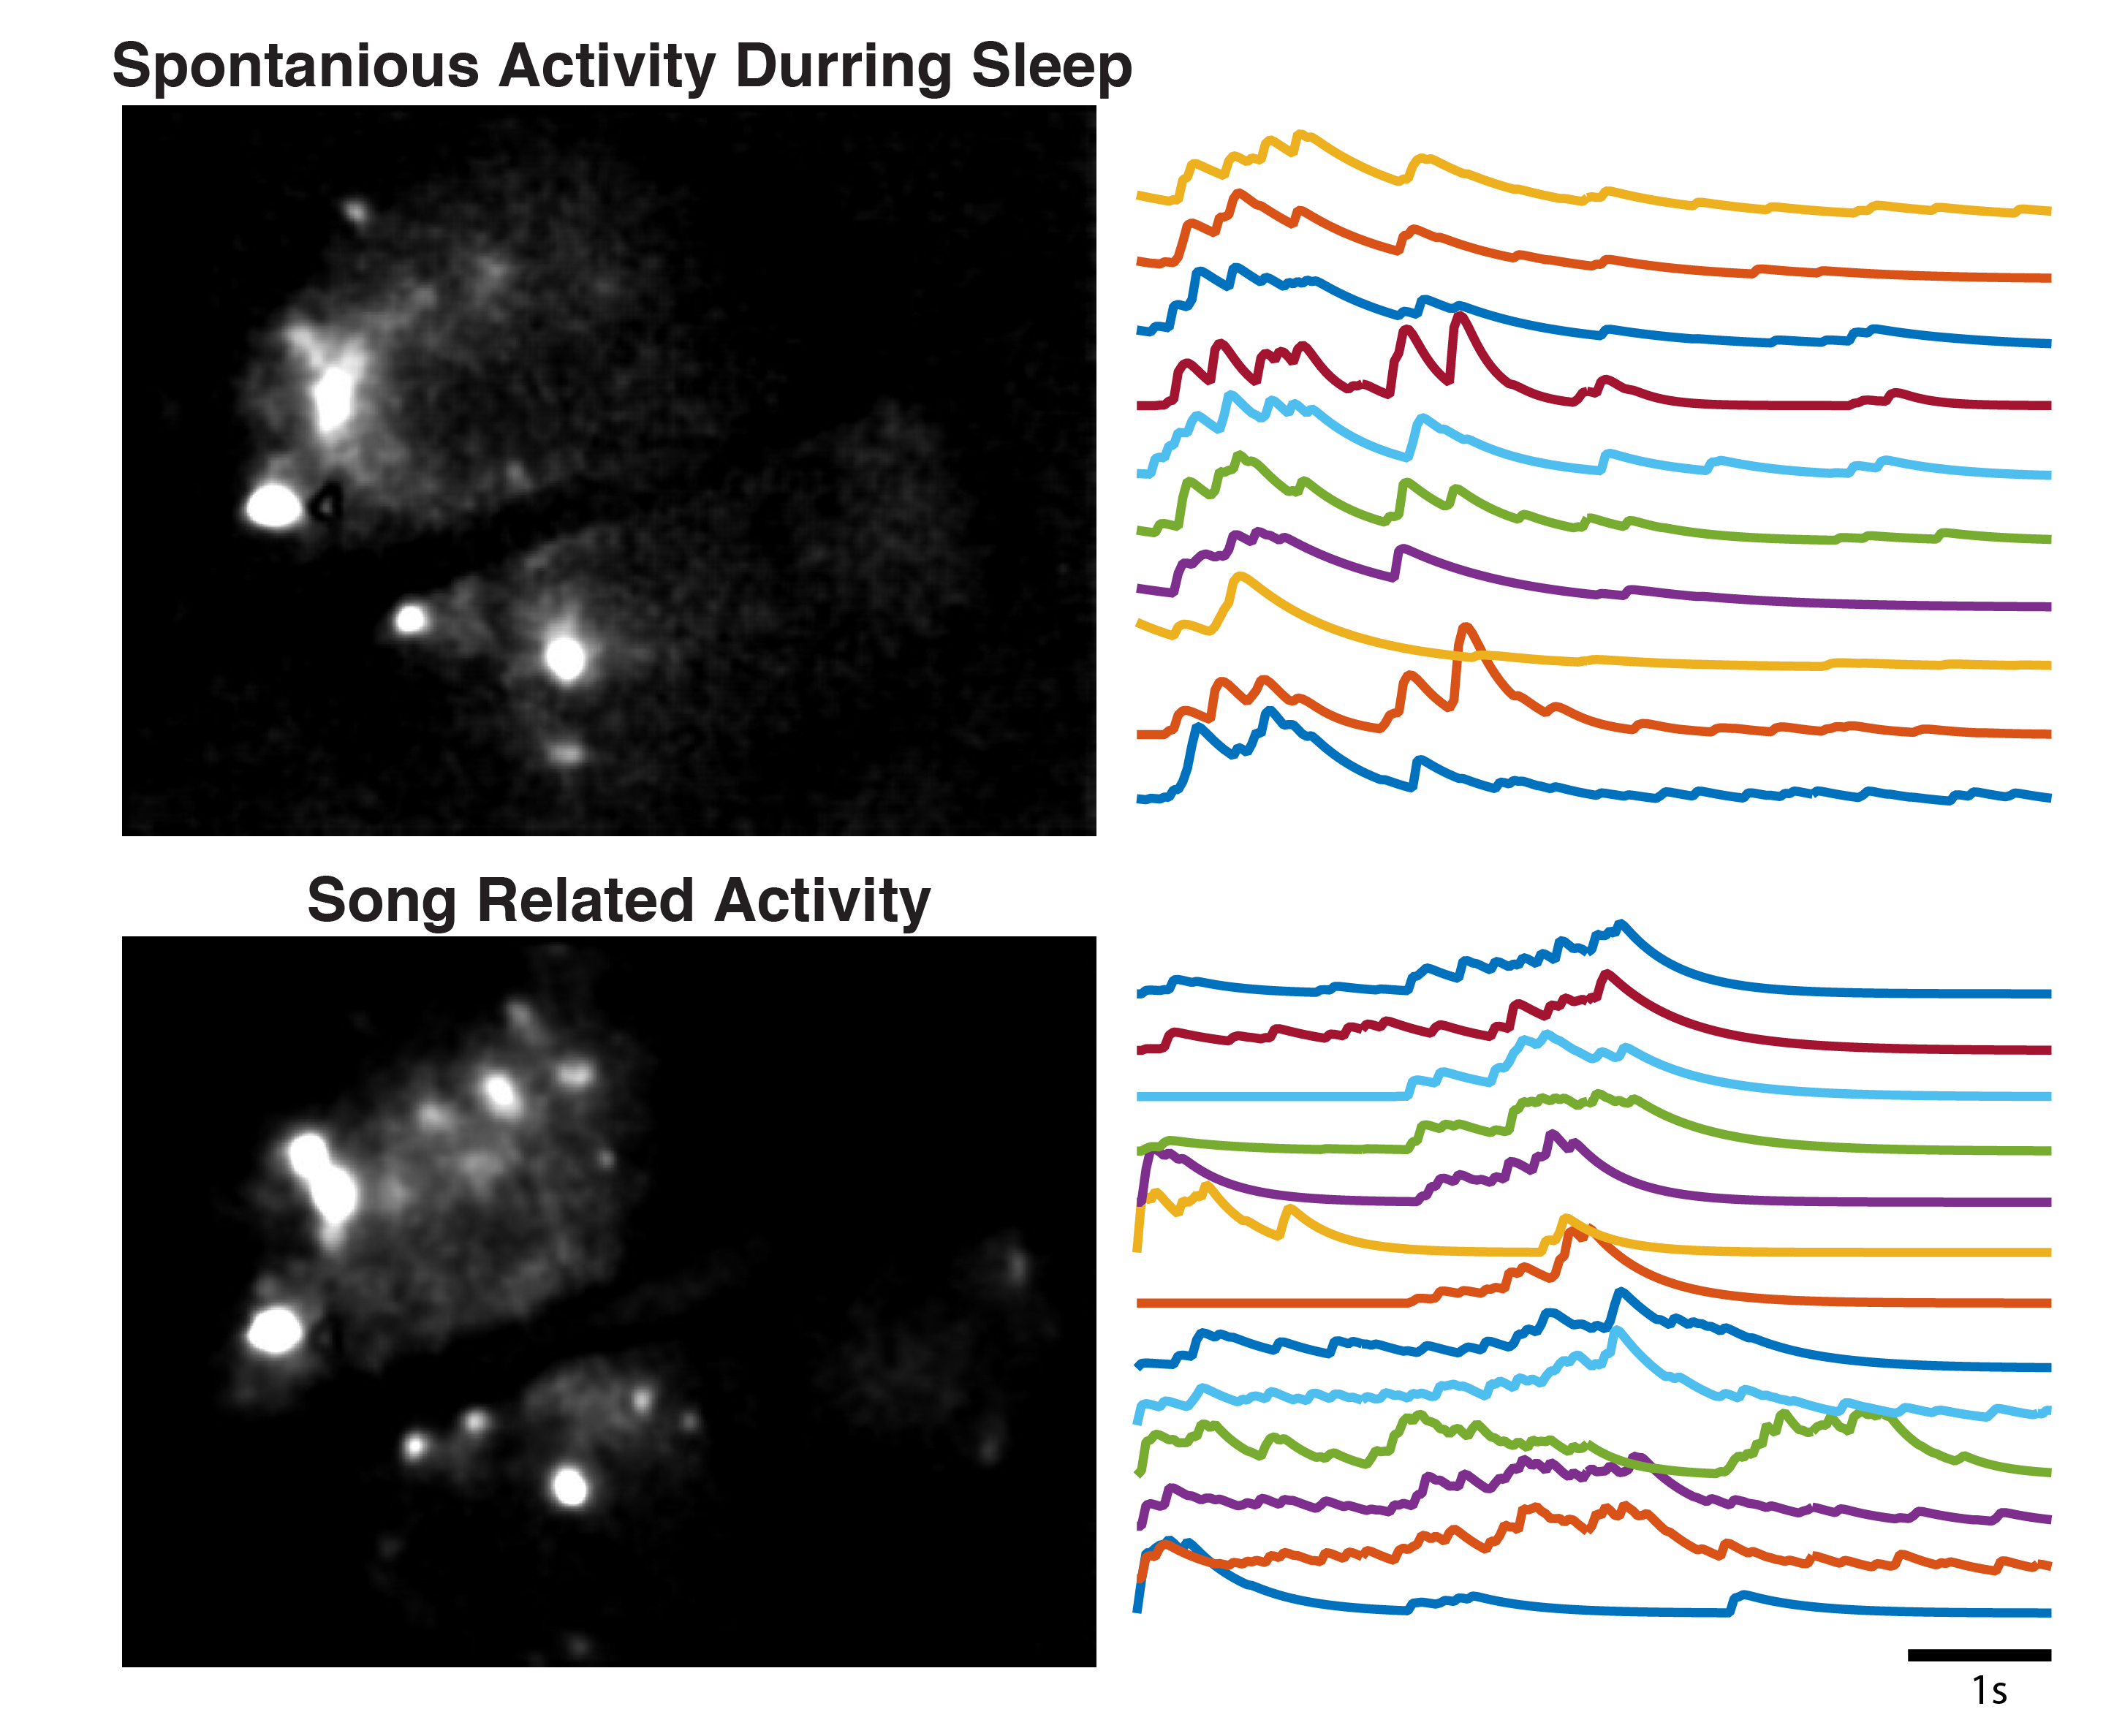
\includegraphics[width=11cm]{figure6.png}
    \centering
\medskip
\caption[Spontaneous activity during sleep]{\footnotesize  \textbf{Spontaneous activity during sleep} \textit{Top}, activity during sleep, contrasted with \textit{Bottom}, song related neural activity. }
\label{fig:Sampling}
\end{figure}
 
During sensorimotor learning of song in juvenile zebra finches, improvements in structure from the previous day deteriorated over a night of sleep, but through the following day improved and surpassed the previous day's quality. Interestingly, juveniles that showed the most 'backsliding' as a result of sleep, achieved the best tutor song imitation as adults (Der�gnaucourt et al. 2005). In addition, spontaneous activity during sleep in juvenile male zebra finches was correlated to the quality of tutor song imitation (Gobes, Zandbergen, and Bolhuis 2010). In the adult, spontaneous neuronal activation during sleep in several parts of the song system appear to resemble motor activation patterns that drive song (Dave and Margoliash 2000). Moreover, there is evidence that noisy or partially incomplete  spontaneous sequence reactivations of the motor plan occur during sleep in the motor region RA(Shank and Margoliash 2009). Taken as a whole, there is strong evidence that sleep plays a role in memory formation in songbirds and that this may be critical for the learning and maintenance of song. (Gobes, Zandbergen, and Bolhuis 2010; Gobes and Bolhuis 2008)

Future experiments are needed to robustly answer how sleep is involved in motor stability and planning. I believe that the zebra finch will presents itself as an ideal model system for addressing these questions; the extreme precision and long-term stability of song structure offers a unique opportunity to observe how motor memories are maintained at the network level- and how these networks are shaped by different states, like sleep. Using cell-type specific genetically encoded calcium indicators and custom miniature head-mounted microscopes, neural populations can be observed over weeks and months. Combining the use of near real-time behavioral and neurally guided feedback mentioned in the previous section, along with round-the-clock monitoring of neural activity will help elucidate the learning roles of individual cells the lead to stable memories.

 




